\documentclass{beamer}
\usepackage{amsmath} % flere matematikkommandoer
\usepackage{amssymb} % flere matematikkommandoer
\usepackage{amsfonts}              % for blackboard bold, etc
\usepackage{amsthm}                % better theorem environments
\usepackage{listings}
\usepackage{graphicx}              % to include figures
\usepackage{tikz}
\usetikzlibrary{arrows,automata,fit,positioning, shapes, arrows.meta,chains,matrix,decorations.pathreplacing, calc}

\newcommand\doubleplus{+\kern-1.3ex+\kern0.8ex}
\newcommand\lett{\phantom{-}\:\:\mathbf{let}\:\:}
\newcommand\inn{\:\:\mathbf{in}\:\:}

\title{Implementing Map-Scan Fusion in the Futhark Compiler}
\author{Brian Spiegelhauer \&  William Sprent}
\institute{DIKU \\ University of Copenhagen}
\date{June 21, 2016}
\begin{document}
\lstset{language=C, frame=single, numbers=left, breaklines=true}
\frame{\titlepage}
\section[intro]{Introduction}
\begin{frame}
\frametitle{Table of Contents}
\tableofcontents[currentsection]
\end{frame}

\begin{frame}
  \frametitle{Introduction}
  \begin{itemize}
  \item Performance increases on hardware increasingly comes from parallisation.
  \item GPUs present an opportunity for massive parallelism.
  \item GPGPU libraries can be low level and cumbersome.
  \item Increasing need for high performance parallel languages.
  \end{itemize}
\end{frame}

\begin{frame}
  \frametitle{Futhark}
\large \textbf{Futhark is:}
\begin{itemize}
\item Functional language with GPU execution.
\item Uses Second Order Array Combinators for bulk array operations.
\item Aggressive optimisation strategy.
\end{itemize}
\end{frame}

\begin{frame}
  \frametitle{SOACs}
  \begin{itemize}
  \item \texttt{map}, \texttt{reduce}, \texttt{scan}, \texttt{filter} etc.
  \item Equivalent to higher-order functions found in functional programming.
  \item Can have strong invariants. Useful with regards to parallelisation, and optimisation.
  \end{itemize}
  \begin{align*}
    &\mathtt{map} \: f \: a \: :  \: (\alpha \to \beta) \to [\alpha] \to [\beta]\\
    &\equiv  \: [f(a_0), f(a_1), ..., f(a_{n-1})]
  \end{align*}
  \begin{align*}
&\mathtt{scan} \: \odot \: e \: a \: : \:(\alpha \to \alpha \to \alpha) \to \alpha \to [\alpha] \to [\alpha] \\
&\equiv [e \odot a_0, e \odot a_0 \odot a_1, ..., e \odot a_0 \odot ... \odot a_{n-1}]
\end{align*}
\end{frame}

\section[fus]{Fusion}

\begin{frame}
\frametitle{Table of Contents}
\tableofcontents[currentsection]
\end{frame}

\begin{frame}
  \frametitle{Loop Fusion}
\large \textbf{Why loop fusion?}
\begin{itemize}
\item Combining loops reduces overhead.
\item Can optimize memory access patterns.
\item Can do away with intermediate arrays.
\end{itemize}
\large \textbf{On GPU -- high penalties for global memory accesses.}
\end{frame}

\begin{frame}[fragile]
  \frametitle{Example}
\begin{lstlisting}[caption=Producer-Consumer pre-fusion.,label={lst:pc-pre}] 
  a[n];
  b[n];
  for (int i = 0; i < n; i++) {
    b[i] = f(a[i]);
  }
  c[n];
  for (int i = 0; i < n; i++) {
    c[i] = g(b[i]);
  }
\end{lstlisting}
\end{frame}

\begin{frame}[fragile]
  \frametitle{Example}
\begin{lstlisting}[caption=Producer-Consumer post-fusion.,label={lst:pc-post}] 
  a[n];
  c[n];

  for (int i = 0; i < n; i++) {
    c[i] = f(g(a[i])
  }
\end{lstlisting}
\end{frame}


\begin{frame}
  \frametitle{Fusing SOACs}

\large \textbf{Why?}
  \begin{itemize}
  \item SOACs express easily as loops.
  \item Compatible SOACs can be fused using simple function composition.
  \item No difficult loop-dependency analysis required!
  \end{itemize}

\large \textbf{How?}
\begin{itemize}
\item Analyse SOAC inter-compatibility for fusion.
\item Express generalised rules for fusing combinations of SOACS.
\end{itemize}
\end{frame}

\begin{frame}
  \frametitle{Previous Example Revisited}
  \begin{align*}
   \lett b &= \mathtt{map} \: f \: a \inn \\
   \lett c &= \mathtt{map} \: g \: b \inn \\
    &\Downarrow \\
    \lett c &= \mathtt{map} \: (g \circ f) \: a \inn 
 \end{align*}
\end{frame}

\begin{frame}
  \frametitle{Map-Scan fusion.}
\large \textbf{Naive approach:}
\begin{align*}
  b &= \mathtt{map} \: f \: a \\
  c &= \mathtt{scan} \: \odot \: e \: b \\
    &\Downarrow \\
  c &= \mathtt{scan} \: \odot_f \: e \: a
\end{align*}
\large \textbf{Problem: Scan requires an associative function.}
\end{frame}


\begin{frame}

 \frametitle{Computing Scan}
 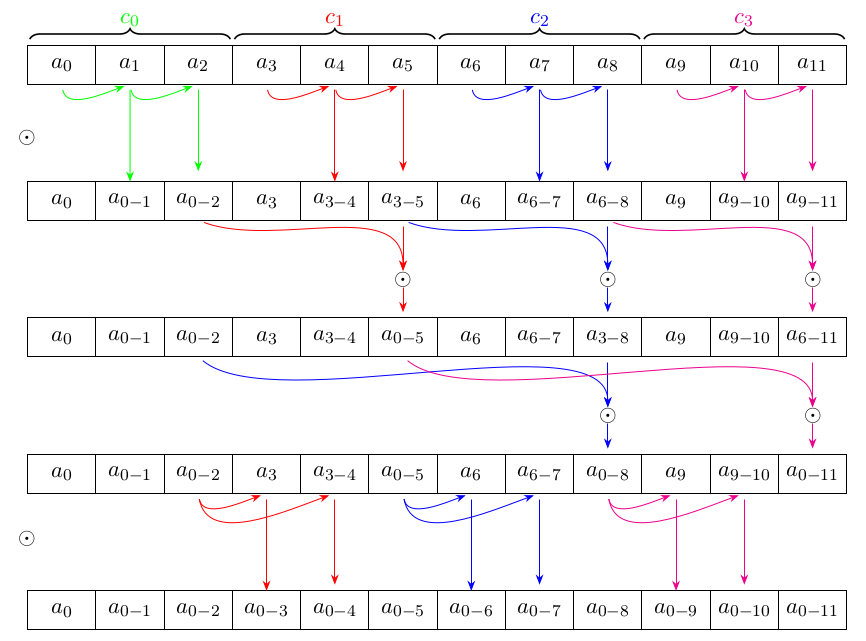
\includegraphics[height=0.7\textheight]{image/monster.png}
\end{frame}


\begin{frame}

 \frametitle{Scanomap}
\large \textbf{Solution:}
 \begin{itemize}
 \item Look at how chunks are computed sequentially.
 \item Extend Scan with a sequential folding function.
 \end{itemize}
 \begin{align*}
   &\mathtt{scanomap} \: \odot \: \odot_f \: e \: a \: \\ &: \:(\alpha \to \alpha \to \alpha) \to (\alpha \to \beta \to \alpha)
 \to \alpha \to [\beta] \to [\alpha] \\
&\equiv
 [e \odot_f a_0, (e \odot_f a_0) \odot_f a_1, ..., ((e \odot_f a_0) \odot_f ...) \odot_f a_{n-1}]
 \end{align*}
\end{frame}


\begin{frame}

 \frametitle{Map-Scan Fusion}
\large \textbf{Using Scanomap to perform Map-Scan fusion:}
\begin{align*}
  b &= \mathtt{map} \: f \: a \\
  c &= \mathtt{scan} \: \odot \: e \: b \\
&\Downarrow \\
  c &= \mathtt{scanomap} \: \odot \: \odot \: e \: b \\
&\Downarrow \\
  c &= \mathtt{scanomap} \: \odot \: \odot_f \: e \: a\mathnormal{.}
\end{align*}
\end{frame}
\section[impl]{Results}
\begin{frame}
\frametitle{Table of Contents}
\tableofcontents[currentsection]
\end{frame}

\begin{frame}
 \frametitle{What have we done?}
 \begin{itemize}
 \item Extended Futhark's internal representation with Scanomap.
 \item Added support for Scanomap in the type-checker, interpreter, SOAC module etc.
 \item Added rules for converting Scanomap into sequential loops.
 \item Extended the fusion module with fusion logic for Scanomap fusions.
 \end{itemize}
\end{frame}

\begin{frame}[fragile]
 \frametitle{Benchmark: Simple Map-Scan}
\begin{lstlisting}
fun ([int]) main([int] inp) =
  let a = map(+10, inp)
  let b = scan(+, 0, a) in
  (b)
\end{lstlisting}
\end{frame}

\begin{frame}
 \frametitle{Benchmark: Simple Map-Scan}
    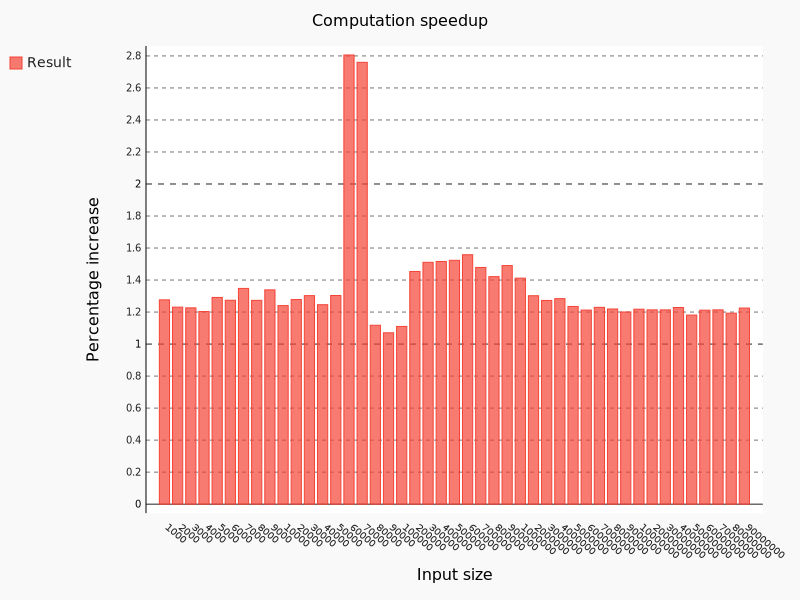
\includegraphics[width=0.9\textwidth]{../images/comparing.png}
\end{frame}

\begin{frame}[fragile]
 \frametitle{Benchmark: Horizontal Fusion}
\begin{lstlisting}
fun [int, n] main([int, n] inp) =
    let a  = map(+10, inp) in
    let b1 = scan(+, 0, a) in
    let a2 = map(+1, a) in
    let b2 = scan(+, 0, a2) in
    map(fn int (int x,int y) => x + y, zip(b1,b2))
\end{lstlisting}
\end{frame}
\begin{frame}
 \frametitle{Benchmark: Horizontal Fusion}
    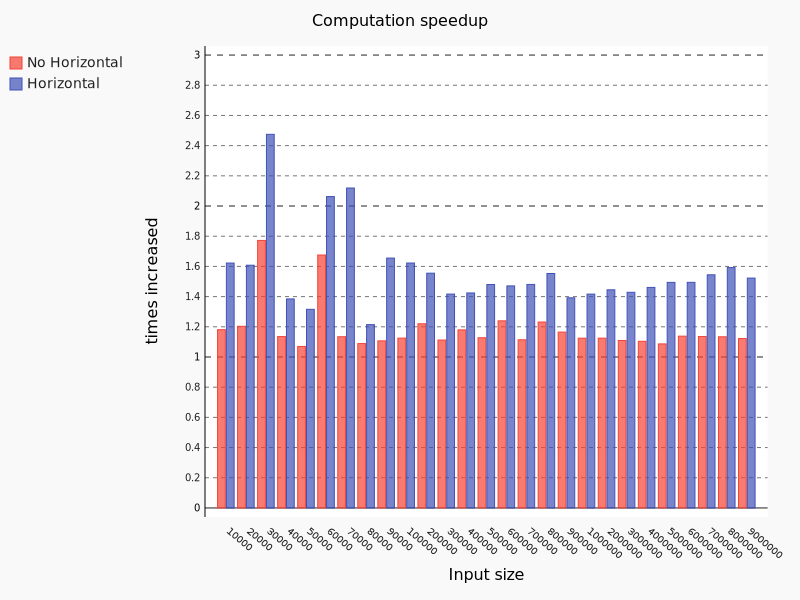
\includegraphics[width=0.9\textwidth]{../images/horri-comparing.png}
\end{frame}
\begin{frame}[fragile]
 \frametitle{Benchmark: Radix Sort}
\begin{lstlisting}
fun [u32, n] radix_sort_step([u32, n] xs, i32 digit_n) =
  let bits = map(fn i32 (u32 x) => i32((x >> u32(digit_n)) & 1u32), xs)
  let bits_inv = map(fn i32 (i32 b) => 1 - b, bits)
  let ps0 = scan(+, 0, bits_inv)
  let ps0_clean = map(*, zip(bits_inv, ps0))
  let ps1 = scan(+, 0, bits)
  let ps0_offset = reduce(+, 0, bits_inv)
  let ps1_clean = map(+ ps0_offset, ps1)
  let ps1_clean' = map(*, zip(bits, ps1_clean))
  let ps = map(+, zip(ps0_clean, ps1_clean'))
  let ps_actual = map(fn i32 (i32 p) => p - 1, ps)
  in write(ps_actual, xs, copy(xs))
\end{lstlisting}
\end{frame}
\begin{frame}
 \frametitle{Benchmark: Radix Sort}
    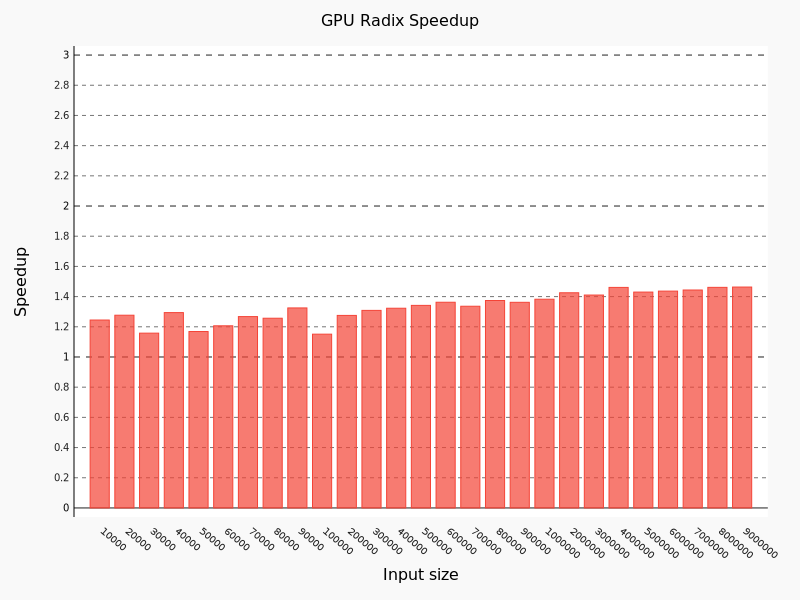
\includegraphics[width=0.9\textwidth]{../images/radix-comparing.png}
\end{frame}

\section[con]{Conclusion}
\begin{frame}
\frametitle{Table of Contents}
\tableofcontents[currentsection]
\end{frame}

\begin{frame}
 \frametitle{Future work}
\large \textbf{Scanomap-Map fusion}
\begin{itemize}
\item Scanomap doesn't natively fuse as a producer.
\item Extend Scanomap with a third function.
\item Fuse with Map using the techniques from earlier.
\end{itemize}
\large \textbf{Should result in similar speedup.}
\end{frame}
\begin{frame}
 \frametitle{Conclusion}
\large \textbf{What have we achieved?}
 \begin{itemize}
 \item Performed Map-Scan fusion using Scanomap.
 \item Implemented further fusion for Scanomap.
 \item Uncovered opportunities for further optimisations.
 \item Demonstrated significant speedup.
 \end{itemize}
\end{frame}
\begin{frame}
\Large End of Presentation.
\end{frame}

\end{document}